\documentclass[12pt]{article}
\usepackage[margin=2cm]{geometry}
\usepackage{amsmath}
\usepackage{slashed}
\usepackage{tikz}

\begin{document}

\noindent
A high energy electron and positron collision can create two muons.
\begin{center}
\begin{tikzpicture}
\draw[dashed] (0,0) circle (0.5cm);
\draw[thick,->] (2,0) node[anchor=west] {$e^+$} -- (0.6,0);
\draw[thick,->] (-2,0) node[anchor=east] {$e^-$} -- (-0.6,0);
\draw[thick,->] (0.40,0.40) -- (1.3,1.3) node[anchor=south west] {$\mu^-$};
\draw[thick,->] (-0.4,-0.4) -- (-1.3,-1.3) node[anchor=north east] {$\mu^+$};
\draw (1,0.5) node {$\theta$};
\end{tikzpicture}
\end{center}

\noindent
Here is the same diagram with momentum and spinor labels.
\begin{center}
\begin{tikzpicture}
\draw[dashed] (0,0) circle (0.5cm);
\draw[thick,->] (2,0) node[anchor=west] {$p_2, v_2$} -- (0.6,0);
\draw[thick,->] (-2,0) node[anchor=east] {$p_1, u_1$} -- (-0.6,0);
\draw[thick,->] (0.40,0.40) -- (1.3,1.3) node[anchor=south west] {$p_3, u_3$};
\draw[thick,->] (-0.4,-0.4) -- (-1.3,-1.3) node[anchor=north east] {$p_4, v_4$};
\draw (1,0.5) node {$\theta$};
\end{tikzpicture}
\end{center}

\noindent
In a typical collider experiment the momentum vectors are
$$
p_1=\begin{pmatrix}E\\0\\0\\p\end{pmatrix}\qquad
p_2=\begin{pmatrix}E\\0\\0\\-p\end{pmatrix}\qquad
p_3=\begin{pmatrix}
E\\
\rho\sin\theta\cos\phi\\
\rho\sin\theta\sin\phi\\
\rho\cos\theta
\end{pmatrix}
\qquad
p_4=\begin{pmatrix}
E\\
-\rho\sin\theta\cos\phi\\
-\rho\sin\theta\sin\phi\\
-\rho\cos\theta
\end{pmatrix}
$$

\noindent
where $E$ is beam energy, $p=\sqrt{E^2-m^2}$, $\rho=\sqrt{E^2-M^2}$,
$m$ is electron mass $0.51\,\text{MeV}$,
and $M$ is muon mass $106\,\text{MeV}$.
The spinors are
\begin{gather*}
u_{11}=\begin{pmatrix}E+m\\0\\p\\0\end{pmatrix}\quad
v_{21}=\begin{pmatrix}-p\\0\\E+m\\0\end{pmatrix}\quad
u_{31}=\begin{pmatrix}E+M\\0\\p_3^z\\p_3^x+ip_3^y\end{pmatrix}\quad
v_{41}=\begin{pmatrix}p_4^z\\p_4^x+ip_4^y\\E+M\\0\end{pmatrix}
\\
u_{12}=\begin{pmatrix}0\\E+m\\0\\-p\end{pmatrix}\quad
v_{22}=\begin{pmatrix}0\\p\\0\\E+m\end{pmatrix}\quad
u_{32}=\begin{pmatrix}0\\E+M\\p_3^x-ip_3^y\\-p_3^z\end{pmatrix}\quad
v_{42}=\begin{pmatrix}p_4^x-ip_4^y\\-p_4^z\\0\\E+M\end{pmatrix}
\end{gather*}

\noindent
The last digit in a spinor subscript is 1 for spin up and 2 for spin down.
Note that the spinors are not individually normalized.
Instead, a combined spinor normalization constant $N=(E+m)^2(E+M)^2$
will be used where needed.

\bigskip
\noindent
This is the probability density for muon production.
Symbol $s=(p_1+p_2)^2=4E^2$,
symbol $s_j$ selects the spin of spinor $j$,
and $e$ is electron charge.
\begin{equation*}
|\mathcal{M}(s_1,s_2,s_3,s_4)|^2
=\frac{e^4}{s^2}\frac{1}{N}\left|(\bar{u}_3\gamma_\mu v_4)(\bar{v}_2\gamma^\mu u_1)\right|^2
\end{equation*}

\noindent
The expected probability density $\langle|\mathcal{M}|^2\rangle$
is computed by summing $|\mathcal{M}|^2$ over all spin states
and dividing by the number of inbound states.
There are four inbound states.
\begin{align*}
\langle|\mathcal{M}|^2\rangle
&=\frac{1}{4}\sum_{s_1=1}^2\sum_{s_2=1}^2\sum_{s_3=1}^2\sum_{s_4=1}^2|\mathcal{M}(s_1,s_2,s_3,s_4)|^2
\\
&=\frac{e^4}{4s^2}\sum_{s_1=1}^2\sum_{s_2=1}^2\sum_{s_3=1}^2\sum_{s_4=1}^2
\frac{1}{N}\left|(\bar{u}_3\gamma_\mu v_4)(\bar{v}_2\gamma^\mu u_1)\right|^2
\end{align*}

\noindent
Another way to compute $\langle|\mathcal{M}|^2\rangle$ is to use the Casimir trick.
\begin{equation*}
\langle|\mathcal{M}|^2\rangle
=\frac{e^4}{4s^2}
\mathop{\rm Tr}\left((\slashed{p}_3+M)\gamma^\mu(\slashed{p}_4-M)\gamma^\nu\right)
\mathop{\rm Tr}\left((\slashed{p}_2-m)\gamma_\mu(\slashed{p}_1+m)\gamma_\nu\right)
\end{equation*}

\noindent
Here is a third way to compute $\langle|\mathcal{M}|^2\rangle$.
\begin{equation*}
\langle|\mathcal{M}|^2\rangle
=\frac{e^4}{4s^2}
\left(
32 (p_1\cdot p_3) (p_2\cdot p_4) +
32 (p_1\cdot p_4) (p_2\cdot p_3) +
32 m^2 (p_3\cdot p_4) +
32 M^2 (p_1\cdot p_2) +
64 m^2 M^2
\right)
\end{equation*}

\noindent
For the momentum vectors given above the result is
\begin{equation*}
\langle|\mathcal{M}|^2\rangle
=e^4\left(1+\cos^2\theta+\frac{m^2+M^2}{E^2}\sin^2\theta+\frac{m^2M^2}{E^4}\cos^2\theta\right)
\end{equation*}

\noindent
The Stanford Linear Collider
had a collision energy of $2E=91$~GeV.
For beam energies such as SLC where $E\gg M$ the above equation can be approximated as
$$
\langle|\mathcal{M}|^2\rangle=e^4(1+\cos^2\theta)
$$

\noindent
The differential cross section is
$$
\frac{d\sigma}{d\Omega}
=\frac{\langle|\mathcal{M}|^2\rangle}{64\pi^2s}
=\frac{e^4}{256\pi^2E^2}(1+\cos^2\theta)
$$

\noindent
Recall that $e^2=4\pi\alpha$ hence
\begin{equation*}
\frac{d\sigma}{d\Omega}=\frac{\alpha^2}{16E^2}(1+\cos^2\theta)
\end{equation*}

\noindent
The total cross section calculation requires the following definite integral.
$$
\int_\Omega(1+\cos^2\theta)\,d\Omega
=\int_0^{2\pi}\int_0^\pi(1+\cos^2\theta)\sin\theta\,d\theta\,d\phi
=\frac{8}{3}\int_0^{2\pi}d\phi
=\frac{16\pi}{3}
$$

\noindent
Hence the total cross section is
$$
\sigma
=\int_\Omega d\sigma
=\int_\Omega\frac{\alpha^2}{16E^2}(1+\cos^2\theta)\,d\Omega
=\frac{\alpha^2}{16E^2}\frac{16\pi}{3}
=\frac{\pi\alpha^2}{3E^2}
$$

\noindent
We can integrate the differential cross section to obtain a cumulative distribution function.

\bigskip
\noindent
Let
\begin{equation*}
I(\xi)=2\pi\int_0^\xi\frac{d\sigma}{d\Omega}\,\sin\theta\,d\theta,
\qquad0\le\xi\le\pi
\end{equation*}

\noindent
The result is
\begin{equation*}
I(\xi)=2\pi\left(\frac{\alpha^2}{16E^2}\right)
\left(-\frac{1}{3}\cos^3\xi-\cos\xi+\frac{4}{3}\right)
\end{equation*}

\noindent
The cumulative distribution function is
\begin{equation*}
F(\theta)=\frac{I(\theta)}{I(\pi)},\qquad0\le\theta\le\pi
\end{equation*}

\noindent
Hence
\begin{equation*}
P(\theta_1\le\theta\le\theta_2)=F(\theta_2)-F(\theta_1)
\end{equation*}

\noindent
The normalized probability density is
\begin{equation*}
f(\theta)=\frac{dF(\theta)}{d\theta}=\frac{3}{8}(1+\cos^2\theta)\sin\theta,
\qquad0\le\theta\le\pi
\end{equation*}

\noindent
Run ``muon-production-5.txt'' to draw the probability density function.

\begin{center}
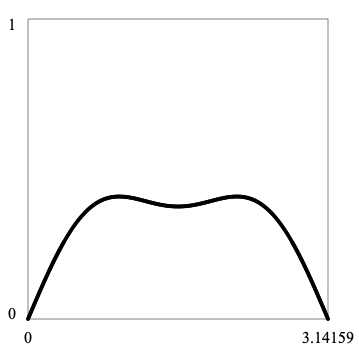
\includegraphics[scale=0.5]{muon-production.png}
\end{center}

\noindent
Run ``muon-production-1.txt'' to verify that
$$
\frac{1}{N}\sum_{s_1=1}^2\sum_{s_2=1}^2\sum_{s_3=1}^2\sum_{s_4=1}^2
\left|(\bar{u}_3\gamma_\mu v_4)(\bar{v}_2\gamma^\mu u_1)\right|^2
=
\mathop{\rm Tr}\left((\slashed{p}_3+M)\gamma^\mu(\slashed{p}_4-M)\gamma^\nu\right)
\mathop{\rm Tr}\left((\slashed{p}_2-m)\gamma_\mu(\slashed{p}_1+m)\gamma_\nu\right)
$$

\bigskip
\noindent
Run ``muon-production-2.txt'' to verify that
\begin{multline*}
\frac{1}{64E^4}
\mathop{\rm Tr}\left((\slashed{p}_3+M)\gamma^\mu(\slashed{p}_4-M)\gamma^\nu\right)
\mathop{\rm Tr}\left((\slashed{p}_2-m)\gamma_\mu(\slashed{p}_1+m)\gamma_\nu\right)
\\
=1+\cos^2\theta+\frac{m^2+M^2}{E^2}\sin^2\theta+\frac{m^2M^2}{E^4}\cos^2\theta
\end{multline*}

\noindent
and to verify that
\begin{multline*}
\mathop{\rm Tr}\left((\slashed{p}_3+M)\gamma^\mu(\slashed{p}_4-M)\gamma^\nu\right)
\mathop{\rm Tr}\left((\slashed{p}_2-m)\gamma_\mu(\slashed{p}_1+m)\gamma_\nu\right)
\\=
32 (p_1\cdot p_3) (p_2\cdot p_4) +
32 (p_1\cdot p_4) (p_2\cdot p_3) +
32 m^2 (p_3\cdot p_4) +
32 M^2 (p_1\cdot p_2) +
64 m^2 M^2
\end{multline*}

\subsection*{Data from SLAC PEP experiment}
See www.hepdata.net/record/ins216031, Table 1, 29.0 GeV.

\begin{center}
\begin{tabular}{|c|c|}
\hline
$x$ & $y$\\
\hline
$-0.925$ & 67.08\\
$-0.85\phantom{0}$ & 58.67\\
$-0.75\phantom{0}$ & 54.66\\
$-0.65\phantom{0}$ & 51.72\\
$-0.55\phantom{0}$ & 43.70\\
$-0.45\phantom{0}$ & 41.12\\
$-0.35\phantom{0}$ & 39.71\\
$-0.25\phantom{0}$ & 35.34\\
$-0.15\phantom{0}$ & 33.35\\
$-0.05\phantom{0}$ & 34.69\\
$\phantom{+}0.05\phantom{0}$ & 34.05\\
$\phantom{+}0.15\phantom{0}$ & 34.48\\
$\phantom{+}0.25\phantom{0}$ & 34.66\\
$\phantom{+}0.35\phantom{0}$ & 35.23\\
$\phantom{+}0.45\phantom{0}$ & 35.60\\
$\phantom{+}0.55\phantom{0}$ & 40.13\\
$\phantom{+}0.65\phantom{0}$ & 42.56\\
$\phantom{+}0.75\phantom{0}$ & 46.37\\
$\phantom{+}0.85\phantom{0}$ & 49.28\\
$\phantom{+}0.925$ & 55.70\\
\hline
\end{tabular}
\end{center}

\noindent
Data $x$ and $y$ have the following relationship with cross section parameters.
\begin{equation*}
x=\cos\theta
\qquad
y=(2E)^2\frac{d\sigma}{d\cos\theta}
\end{equation*}

\noindent
The differential cross section for muon production is
\begin{equation*}
\frac{d\sigma}{d\Omega}=\frac{\alpha^2}{16E^2}(1+\cos^2\theta)
\end{equation*}

\noindent
Let us compute predicted values $\hat{y}$ from the cross section formula.
Start by finding the relationship between $d\Omega$ and $d\cos\theta$.
Since $1+\cos^2\theta$ has no dependence on $\phi$ we have
\begin{equation*}
\int_\Omega(1+\cos^2\theta)\,d\Omega
=\int_0^{2\pi}\int_0^{\pi}(1+\cos^2\theta)\sin\theta\,d\theta\,d\phi
=2\pi\int_0^\pi(1+\cos^2\theta)\sin\theta\,d\theta
\end{equation*}

\noindent
Hence
\begin{equation*}
d\Omega=2\pi\sin\theta\,d\theta=-2\pi\,d\cos\theta
\end{equation*}

\noindent
We want positive cross sections so drop the minus sign and set
\begin{equation*}
\frac{d\sigma}{d\cos\theta}=2\pi\frac{d\sigma}{d\Omega}
\end{equation*}

\noindent
We can now write
\begin{align*}
y&=(2E)^2\frac{d\sigma}{d\cos\theta}\\
&=(2E)^2(2\pi)\frac{d\sigma}{d\Omega}\\
&=(2E)^2(2\pi)\frac{\alpha^2}{16E^2}(1+\cos^2\theta)\\
&=\frac{\pi\alpha^2}{2}(1+\cos^2\theta)
\end{align*}

\noindent
Multiply by $(\hbar c)^2$ to convert to SI
and multiply by $10^{37}$ to convert square meters to nanobarns.
\begin{equation*}
y=\frac{\pi\alpha^2}{2}(1+\cos^2\theta)\times(\hbar c)^2\times10^{37}
\end{equation*}

\noindent
Replace $\cos\theta$ with explanatory variable $x$ to obtain $\hat{y}$.
\begin{equation*}
\hat{y}=\frac{\pi\alpha^2}{2}(1+x^2)\times(\hbar c)^2\times10^{37}
\end{equation*}

\noindent
Here are the predicted values $\hat{y}$ based on the above formula.

\begin{center}
\begin{tabular}{|c|c|c|}
\hline
$x$ & $y$ & $\hat{y}$ \\
\hline
$-0.925$ & 67.08 & 60.44\\
$-0.85\phantom{0}$ & 58.67 & 56.10\\
$-0.75\phantom{0}$ & 54.66 & 50.89\\
$-0.65\phantom{0}$ & 51.72 & 46.33\\
$-0.55\phantom{0}$ & 43.70 & 42.42\\
$-0.45\phantom{0}$ & 41.12 & 39.17\\
$-0.35\phantom{0}$ & 39.71 & 36.56\\
$-0.25\phantom{0}$ & 35.34 & 34.61\\
$-0.15\phantom{0}$ & 33.35 & 33.30\\
$-0.05\phantom{0}$ & 34.69 & 32.65\\
$\phantom{+}0.05\phantom{0}$ & 34.05 & 32.65\\
$\phantom{+}0.15\phantom{0}$ & 34.48 & 33.30\\
$\phantom{+}0.25\phantom{0}$ & 34.66 & 34.61\\
$\phantom{+}0.35\phantom{0}$ & 35.23 & 36.56\\
$\phantom{+}0.45\phantom{0}$ & 35.60 & 39.17\\
$\phantom{+}0.55\phantom{0}$ & 40.13 & 42.42\\
$\phantom{+}0.65\phantom{0}$ & 42.56 & 46.33\\
$\phantom{+}0.75\phantom{0}$ & 46.37 & 50.89\\
$\phantom{+}0.85\phantom{0}$ & 49.28 & 56.10\\
$\phantom{+}0.925$ & 55.70 & 60.44\\
\hline
\end{tabular}
\end{center}

\noindent
The coefficient of determination $R^2$ measures how well predicted values fit the real data.
\begin{equation*}
R^2=1-\frac{\sum(y-\hat{y})^2}{\sum(y-\bar{y})^2}=0.87
\end{equation*}

\noindent
The result indicates that the model $d\sigma$ explains 87\% of the variance in the data.

\bigskip
\noindent
Run ``muon-production-3.txt'' to compute the above results.

\subsection*{Electroweak model}
The following differential cross section formula from electroweak
theory results in a better fit to the
data.\footnote{F. Mandl and G. Shaw, {\it Quantum Field Theory Revised Edition,} 316.}

\begin{equation*}
\frac{d\sigma}{d\Omega}=F(s)(1+\cos^2\theta)+G(s)\cos\theta
\end{equation*}

\noindent
where
\begin{align*}
F(s)&=\frac{\alpha^2}{4s}
\left(
1+\frac{g_V^2}{\sqrt{2}\pi}\left(\frac{m_Z^2}{s-m_Z^2}\right)\left(\frac{sG}{\alpha}\right)
+\frac{(g_A^2+g_V^2)^2}{8\pi^2}\left(\frac{m_Z^2}{s-m_Z^2}\right)^2\left(\frac{sG}{\alpha}\right)^2
\right)
\\
G(s)&=\frac{\alpha^2}{4s}
\left(
\frac{\sqrt{2}g_A^2}{\pi}\left(\frac{m_Z^2}{s-m_Z^2}\right)\left(\frac{sG}{\alpha}\right)
+\frac{g_A^2g_V^2}{\pi^2}\left(\frac{m_Z^2}{s-m_Z^2}\right)^2\left(\frac{sG}{\alpha}\right)^2
\right)
\end{align*}

\noindent
and
\begin{align*}
g_A&=-0.5
\\
g_V&=-0.0348
\\
m_Z&=91.17\,\text{GeV}
\\
G&=1.166\times10^{-5}\,\text{GeV}^{-2}
\end{align*}

\noindent
The corresponding formula for $\hat{y}$ is
\begin{equation*}
\hat{y}=2\pi\left[F(s)(1+x^2)+G(s)x\right]\times(\hbar c)^2\times10^{37}
\end{equation*}

\noindent
where $\sqrt{s}=29\,\text{GeV}$ is the center of mass collision energy.
Here are the predicted values $\hat{y}$ based on the above formula.

\begin{center}
\begin{tabular}{|c|c|c|}
\hline
$x$ & $y$ & $\hat{y}$ \\
\hline
$-0.925$ & 67.08 & 65.59\\
$-0.85\phantom{0}$ & 58.67 & 60.84\\
$-0.75\phantom{0}$ & 54.66 & 55.07\\
$-0.65\phantom{0}$ & 51.72 & 49.96\\
$-0.55\phantom{0}$ & 43.70 & 45.49\\
$-0.45\phantom{0}$ & 41.12 & 41.69\\
$-0.35\phantom{0}$ & 39.71 & 38.53\\
$-0.25\phantom{0}$ & 35.34 & 36.02\\
$-0.15\phantom{0}$ & 33.35 & 34.17\\
$-0.05\phantom{0}$ & 34.69 & 32.97\\
$\phantom{+}0.05\phantom{0}$ & 34.05 & 32.42\\
$\phantom{+}0.15\phantom{0}$ & 34.48 & 32.53\\
$\phantom{+}0.25\phantom{0}$ & 34.66 & 33.28\\
$\phantom{+}0.35\phantom{0}$ & 35.23 & 34.69\\
$\phantom{+}0.45\phantom{0}$ & 35.60 & 36.75\\
$\phantom{+}0.55\phantom{0}$ & 40.13 & 39.47\\
$\phantom{+}0.65\phantom{0}$ & 42.56 & 42.83\\
$\phantom{+}0.75\phantom{0}$ & 46.37 & 46.85\\
$\phantom{+}0.85\phantom{0}$ & 49.28 & 51.52\\
$\phantom{+}0.925$ & 55.70 & 55.45\\
\hline
\end{tabular}
\end{center}

\noindent
The coefficient of determination $R^2$ is
\begin{equation*}
R^2=1-\frac{\sum(y-\hat{y})^2}{\sum(y-\bar{y})^2}=0.98
\end{equation*}

\noindent
The result indicates that electroweak theory explains 98\% of the variance in the data.

\bigskip
\noindent
Run ``muon-production-4.txt'' to verify.

\subsection*{Notes}
Here are a few notes about how the scripts work.

\bigskip
\noindent
In component notation the traces become sums over the repeated index $\alpha$.
\begin{align*}
\mathop{\rm Tr}\left((\slashed{p}_3+M)\gamma^\mu(\slashed{p}_4-M)\gamma^\nu\right)
&=
(\slashed{p}_3+M)^\alpha{}_\beta
\gamma^{\mu\beta}{}_\rho
(\slashed{p}_4-M)^\rho{}_\sigma
\gamma^{\nu\sigma}{}_\alpha
\\
\mathop{\rm Tr}\left((\slashed{p}_2-m)\gamma_\mu(\slashed{p}_1+m)\gamma_\nu\right)
&=
(\slashed{p}_2-m)^\alpha{}_\beta
\gamma_\mu{}^\beta{}_\rho
(\slashed{p}_1+m)^\rho{}_\sigma
\gamma_\nu{}^\sigma{}_\alpha
\end{align*}

\noindent
To convert the above formulas to Eigenmath code,
the $\gamma$ tensors need to be transposed
so that repeated indices are adjacent to each other.
Also, multiply $\gamma^\mu$ by the metric tensor to lower the index.
\begin{align*}
\gamma^{\beta\mu}{}_\rho\quad&\rightarrow\quad
\text{\tt gammaT = transpose(gamma)}\\
\gamma^\beta{}_{\mu\rho}\quad&\rightarrow\quad
\text{\tt gammaL = transpose(dot(gmunu,gamma))}
\end{align*}

\noindent
Define the following $4\times4$ matrices.
\begin{align*}
(\slashed{p}_1+m)\quad&\rightarrow\quad\text{\tt X1 = pslash1 + m I}\\
(\slashed{p}_2-m)\quad&\rightarrow\quad\text{\tt X2 = pslash2 - m I}\\
(\slashed{p}_3+M)\quad&\rightarrow\quad\text{\tt X3 = pslash3 + M I}\\
(\slashed{p}_4-M)\quad&\rightarrow\quad\text{\tt X4 = pslash4 - M I}
\end{align*}

\noindent
Then
\begin{align*}
(\slashed{p}_3+M)^\alpha{}_\beta
\gamma^{\mu\beta}{}_\rho
(\slashed{p}_4-M)^\rho{}_\sigma
\gamma^{\nu\sigma}{}_\alpha
\quad&\rightarrow\quad
\text{\tt T1 = contract(dot(X3,gammaT,X4,gammaT),1,4)}
\\
(\slashed{p}_2-m)^\alpha{}_\beta
\gamma_\mu{}^\beta{}_\rho
(\slashed{p}_1+m)^\rho{}_\sigma
\gamma_\nu{}^\sigma{}_\alpha
\quad&\rightarrow\quad
\text{\tt T2 = contract(dot(X2,gammaL,X1,gammaL),1,4)}
\end{align*}

\noindent
Next, multiply matrices and sum over repeated indices.
The dot function sums over $\nu$ then the contract function
sums over $\mu$. The transpose makes the $\nu$ indices adjacent
as required by the dot function.
$$
\mathop{\rm Tr}(\cdots\gamma^\mu\cdots\gamma^\nu)\mathop{\rm Tr}(\cdots\gamma_\mu\cdots\gamma_\nu)
\quad\rightarrow\quad
\text{\tt contract(dot(T1,transpose(T2)))}
$$

\end{document}
